%\chapter{Preliminaries}
\chapter{準備}

\section{RDFについて}
\label{knowlegde:rdf}

\textbf{RDF(Resource Description Framework)}は、WWW上で資源に関する情報を表わすための言語である.
タイトル、著者、ウェブ・ページの更新日、ウェブ・ドキュメントの著作権およびライセンス情報、
ある共有資源に対する利用可能スケジュールなどのような、ウェブ資源に関するメタデータの表現を特に目的としている.
\footnote{http://www.asahi-net.or.jp/~ax2s-kmtn/internet/rdf/rdf-primer}
RDF形式で記述された情報がトリプル(図\ref{fig:rdf_triple}のA)あるいはRDFグラフ(トリプルの集合)(図\ref{fig:rdf_triple}のB)で表現できる.

\begin{figure}[h!]
 	\begin{center}
 		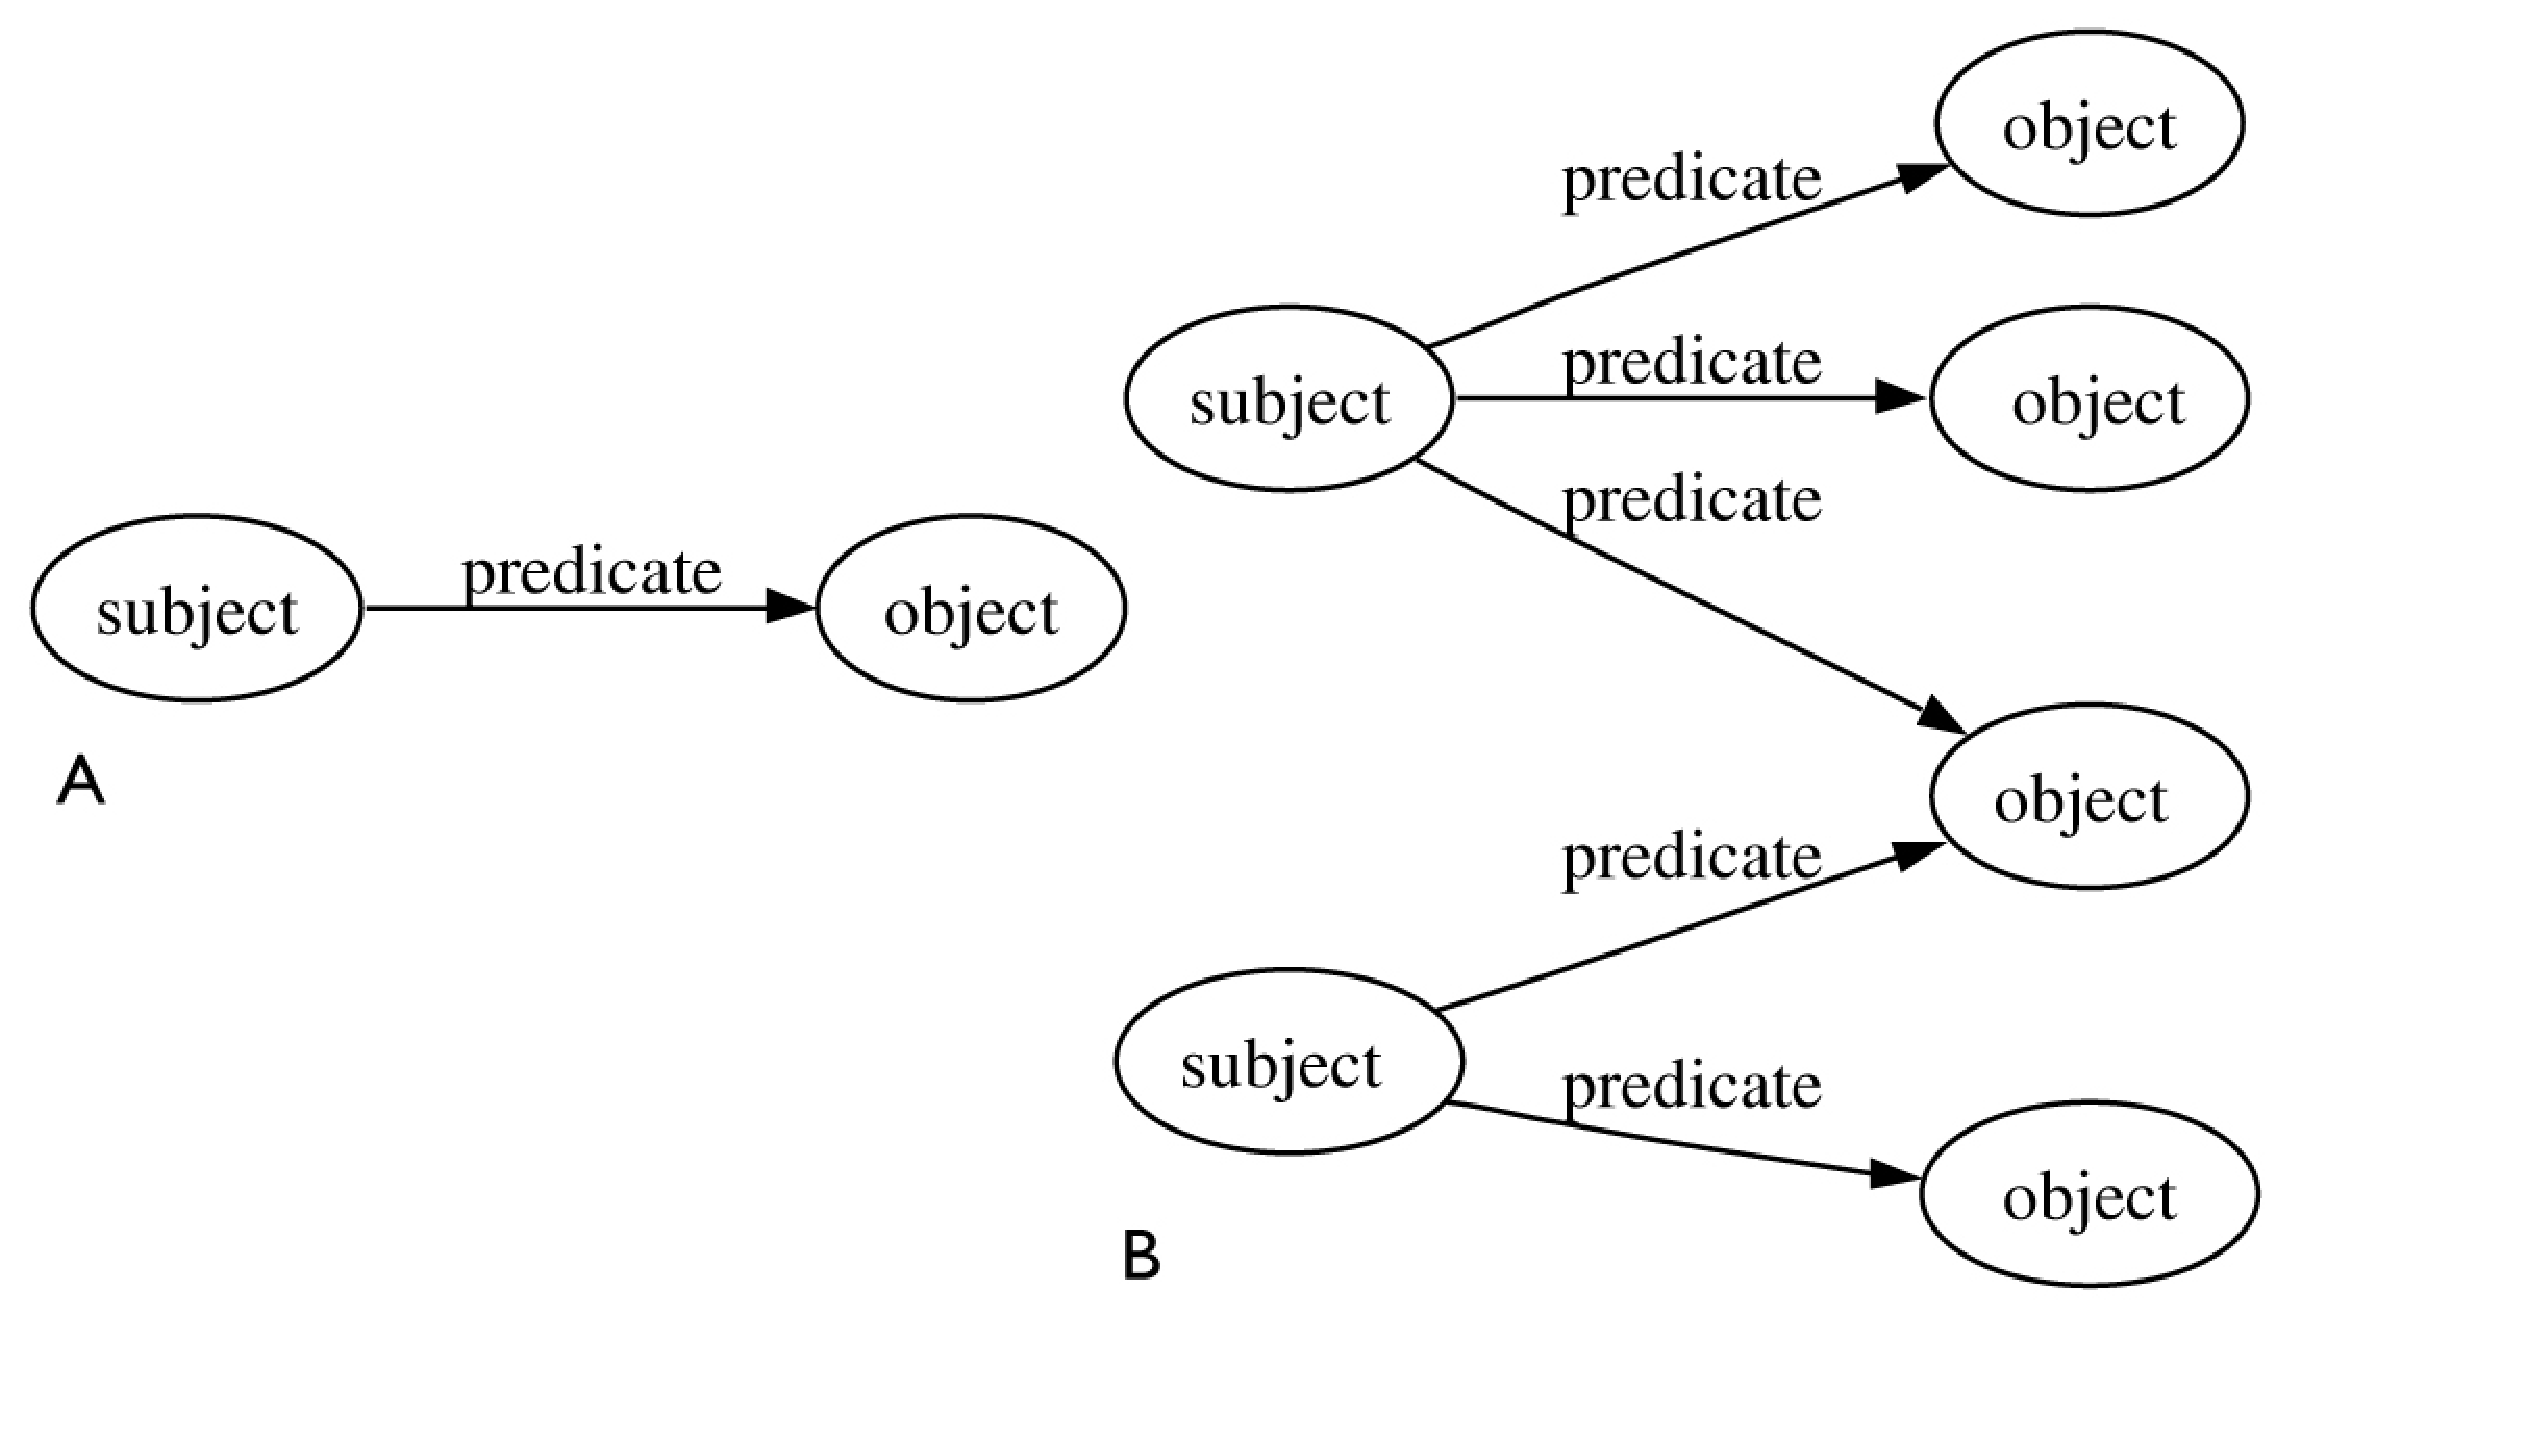
\includegraphics[width=160mm]{./images/rdf_sample.eps}
 		\caption{RDFの例}
 		\label{fig:rdf_triple}
 	\end{center}
\end{figure}

\section{Apache JenaとTDB}

